\documentclass[a4paper]{article}
\usepackage[english]{babel} 
\usepackage[utf8]{inputenc} 

\usepackage{amssymb,amsmath}
\usepackage{enumerate}
\usepackage{enumitem}

\usepackage{graphicx}
\usepackage{color,soul}
\usepackage{xcolor}

\definecolor{mygreen}{rgb}{0,0.6,0}
\definecolor{mygray}{rgb}{0.5,0.5,0.5}
\definecolor{mymauve}{rgb}{0.58,0,0.82}
\definecolor{greenish}{RGB}{105,114,41}

\usepackage[nottoc,numbib]{tocbibind}

\usepackage{xspace}

\usepackage{tikz}
\usetikzlibrary{arrows, automata}

\usepackage{parskip}

\usepackage{lmodern}

\usepackage[
	pdftex,
	pdfauthor={\@author},
	pdftitle={\@title},
	pdfsubject={},
	pdfkeywords={},
	pdfproducer={},
	pdfcreator={}
]{hyperref}
\hypersetup{
	colorlinks,
	linkcolor={red!50!black},
	citecolor={blue!50!black},
	urlcolor={blue!80!black}
}

\usepackage{pgfgantt}
\usepackage{lscape}

\usepackage{listings}

\lstset{
	backgroundcolor=\color{white},   % choose the background color; you must add \usepackage{color} or \usepackage{xcolor}; should come as last argument
	basicstyle=\ttfamily,        % the size of the fonts that are used for the code
	breakatwhitespace=true,          % sets if automatic breaks should only happen at whitespace
	breaklines=true,                 % sets automatic line breaking
	captionpos=b,                    % sets the caption-position to bottom
	commentstyle=\color{mygreen},    % comment style
	frame=single,	                 % adds a frame around the code
	keepspaces=true,                 % keeps spaces in text, useful for keeping indentation of code (possibly needs columns=flexible)
	columns=flexible,
	keywordstyle=\color{blue},   	 % keyword style
	commentstyle=\color{red},
	language=bash,                  % the language of the code
%	numbers=left,                    % where to put the line-numbers; possible values are (none, left, right)
%	numbersep=5pt,                   % how far the line-numbers are from the code
%	numberstyle=\tiny\color{mygray}, % the style that is used for the line-numbers
	rulecolor=\color{black},         % if not set, the frame-color may be changed on line-breaks within not-black text (e.g. comments (green here))
	showstringspaces=false,
	numberstyle=\small,
	stepnumber=1,                    % the step between two line-numbers. If it's 1, each line will be numbered
	stringstyle=\color{mymauve},     % string literal style
	tabsize=2,	                     % sets default tabsize to 2 spaces
	title=\lstname,                  % show the filename of files included with \lstinputlisting; also try caption instead of title
	morekeywords={match, where, return, --}
}

\newcommand{\lstlistshow}[2]{
	\begin{minipage}{\linewidth}
		\lstinputlisting[language=Dockerfile, caption={#2}]{#1}
	\end{minipage}
}

\newcommand{\lstlistdiscuss}[4]{
	\begin{minipage}{\linewidth}
		\lstinputlisting[language=Dockerfile, numbers=left, firstnumber=#2, linerange={#2-#3}, caption={#4}]{#1}
	\end{minipage}
}

\author{Claudio Bonesana}

\title{
	\begin{center}
		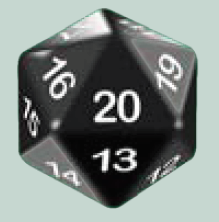
\includegraphics[width=0.4\textwidth]{dice.png}
    \end{center}
    \Large New Techno War \\
	\rule{10cm}{0.3mm} \\
	\large \textit{Guide to the Graphical User Interface} \\
}

\date{Last revision: \today}

\setlength\parindent{0pt}


\begin{document}
	
	\maketitle
	
	% \tableofcontents

	% ---------------------------------------------------------------------------------------------------------

	\section{Introduction}

	This \textit{Web-based Graphical User Interface} (GUI, from now on) is a web application that can be used to view and play against agents built for the project \textit{"New Techno War"}. This application is a prototype and it is \textbf{NOT} a game. In order to speed up the development, we used simple web technologies to display information and let human see and play against the agents.

	\subsection{The project}

	The \textit{"New Techno War"} aims to develop intelligent agents that are capable of play a turn based board game, where different war scenarios are presented. The challenge offered by this game is a dynamic evolution of the game where both attacker and defender need to adapt their strategies to win a scenario.

	If you landed on this page, you will already know everything regarding this project.

	\subsection{Partners}

	This project was developed by \textit{IDSIA} (the Dalle Molle Institute for Studies on Artificial Intelligence) in collaboration with Armasuisse. The board game is produced and developed by Helvetia Games AG.

	\subsection{Technologies and browser compatibility}

	The application was developed completely using modern web technologies such as HTML5, CSS3, and JavaScript. It was tested on modern browser such as Firefox, Chrome, and Edge. Safari and mobile browser compatibility were not tested.

	% ---------------------------------------------------------------------------------------------------------
	
	\section{The lobby}

	\begin{figure}[ht!]
		\centering
		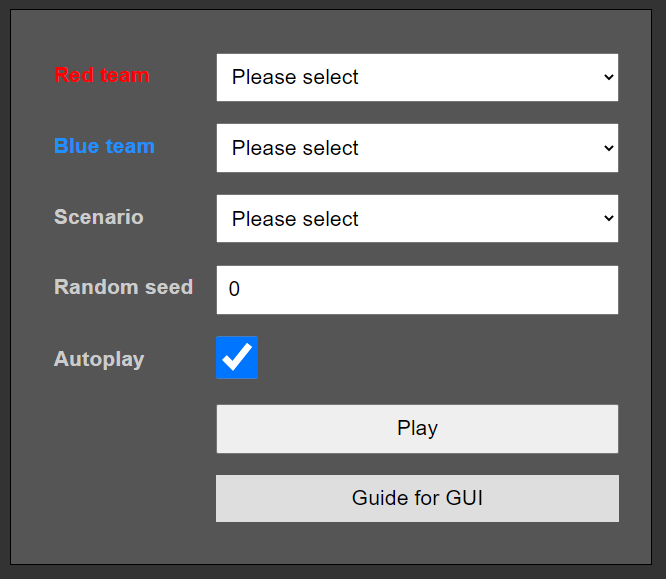
\includegraphics[width=0.75\textwidth]{lobby.png}
		\caption{The lobby page.}
		\label{lobby}
	\end{figure}

	Figure~\ref{lobby} shows the lobby, the first page of the game, where it is possible to choose all the parameters of a game.

	\begin{itemize}
		\item \textbf{Red team}\\ In these scenarios, it is the team that attack and has an intelligence advantage in early game. Use the dropdown menu to choose the kind of agent to use.
		
		\item \textbf{Blue team}\\ In these scenarios, it is the team that defends and has an intelligence advantage in late game. Use the dropdown menu to choose the kind of agent to use.
		
		\item \textbf{Scenario}\\ These scenarios are based on the maps of the board game. Use the dropdown menu to choose the scenario to play on.
		
		\item \textbf{Random seed}\\ The game uses randomness to determine the evolution of a match. Seed controls the possibility to repeat a scenario and have the same evolution multiple times. The value \texttt{0} means that a random seed will be chosen at random. Any other value will be considered a fixed seed.
		
		\item \textbf{Autoplay}\\ If this checkbox is flagged, then the agents controlled by the computer will play during their turn without human interaction. There is a delay of 1.5 second between each action of an agent controlled by the computer in order to let the human understand an action. This delay cannot be changed. Please note that after this delay an agent will start its computation for the next action. This could require some additional time.\\
		Humans agents does not have autoplay since they have to interact.
		
		\item \textbf{Play}\\ Press this button to start the game.
		
		\item \textbf{Guide for GUI}\\ Press this button to read this document.
	\end{itemize}

	% ---------------------------------------------------------------------------------------------------------

	\section{The agents}

	The available agents, in the moment of writing this document, are the following.

	\subsection{Human}
	An interactive player controlled by an human. It is possible to give order to the troops of this team using a mouse.

	\subsection{GreedyAgent}
	An agent played by the computer. It will find the optimal action to perform between the available action to achieve the goal of the scenario.

	% ---------------------------------------------------------------------------------------------------------
	
	\section{The gameboard}

	\begin{figure}[ht!]
		\centering
		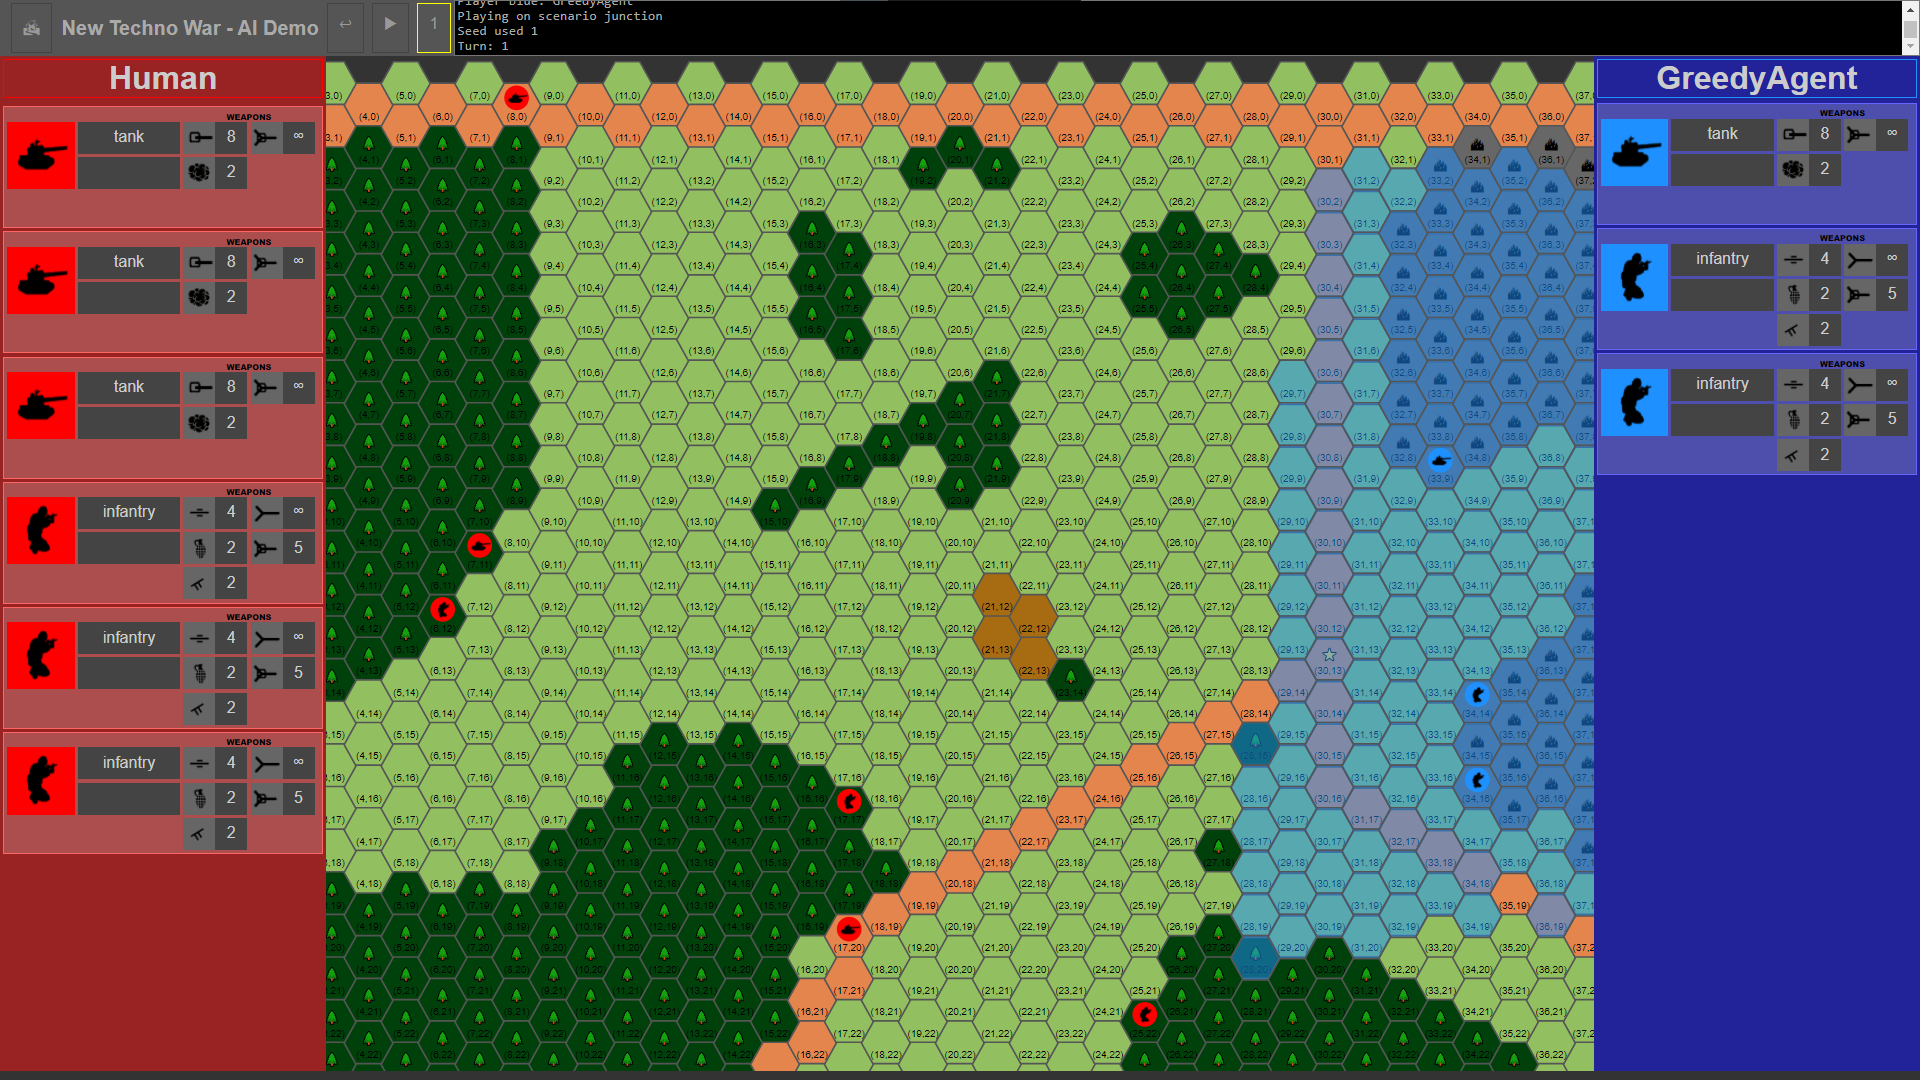
\includegraphics[width=0.75\textwidth]{game.png}
		\caption{The game board.}
		\label{game}
	\end{figure}

	Figure~\ref{game} shows how appears the GUI when a play is in act. If the teams are both controlled by the computer and the \textit{autoplay} flag is checked, there is nothing to do. Enjoy the match.

	\begin{figure}[ht!]
		\centering
		
\includegraphics[width=0.75\textwidth]{controls.png}
		\caption{From left to right: \textit{home} button, \textit{reset} button, \textit{step} button, turn ticker, and game log.}
		\label{controls}
	\end{figure}

	Figure~\ref{controls} shows the available control of the game. These controls are used to move forward, reset a game, or give information regarding the current status of the game.

	\begin{itemize}
		\item \textit{Home button} is used to return to the lobby.
		
		\item \textit{Reset button} can be used to reset the current play to its initial state.
		
		\item \textit{Step button} (or press the \textbf{space bar} on your keyboard) can be used to move to the next step. If the autoplay flag is not set, use this to move forward. This is an important button that can also be used to totally pass when nothing can be done.
		
		Note that an \textit{update} (go from one turn to the next one) is also a step.
		
		\item \textit{Turn ticker} shows the turn we are in. Highlighted in yellow when the turn changes.
		
		\item \textit{Game log} shows information regarding the development of the game. The text in this area can be selected and copied.
	
	\end{itemize}

	% ---------------------------------------------------------------------------------------------------------

	\section{Human interaction}

	When using an \textit{human} agent, it is possible to interact with the game and give order or place units. Human interaction is completely free: there is no check on the validity of moves done by a Human. This capability is intended for testing purposes.

	\subsection{Information panel}

	\begin{figure}[ht!]
		\centering
		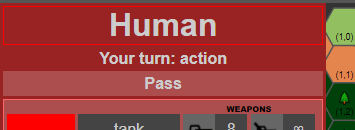
\includegraphics[width=0.75\textwidth]{pass.png}
		\caption{The information panel for a red Human player.}
		\label{infos}
	\end{figure}

	When playing as a human, below the agent name there is an information panel that shows the current action to perform and a \textit{Pass} button that can be used to give a pass order.

	\subsection{Give orders}

	\begin{figure}[ht!]
		\centering
		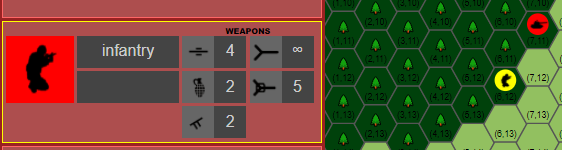
\includegraphics[width=0.75\textwidth]{interactive.png}
		\caption{By moving the mouse over a unit descriptor, the relative unit in the board will be highlighted. To give order interact with the descriptor then on an hexagon on the board (move order) or on the weapon icons then on another unit descriptor (attack order).}
		\label{interactive}
	\end{figure}

	Figure~\ref{interactive} shows the \textit{descriptor} of a unit: this is the box inside the yellow border on the image. When the mouse hovers a descriptor, the border is highlighted in yellow and the relative figure mark is also highlighted in yellow.

	Units with a desaturated colour as descriptor (like in the figure) can perform actions, while units with full saturated colour cannot. This does not include response actions.

	If the GUI does not react to the order, then the order was not performed or it was not valid. Repeat the order to issue a new one.

	If the order is accepted, the GUI will proceed to the next step.

	\subsection{Placement and move command}

	When there is an area on the board with the same colour of an agent, the agent can place units. While computer based agents will perform the placement after the first \textit{step}, human agents can place their units by giving a move command.

	A move command is performed by clicking on a descriptor (pay attention to \textbf{not} click on a weapon) then on a free hexagon on the board. During placement stage, multiple move command can be performed.

	Once placement is done, press the \textit{step} button to start the game.

	\subsection{Attack and responses}

	Attack and response orders are performed in the same way. Click first on the icon of the weapon you want to use, then click on the \textit{descriptor} of an enemy unit. This will perform the action.

	\subsection{Pass}

	Currently there are multiple ways to perform a pass.

	\begin{enumerate}
		\item Click on the \textit{step} button.
		
		\item Click on the \textit{pass} button below the information panel. This can be used to skip responses.
		
		\item Click first on a descriptor of a figure then on the \textit{pass} button. This will give a \textit{pass order} to a specified unit.
	\end{enumerate}

	% ---------------------------------------------------------------------------------------------------------

\end{document}